% Gabarit pandoc des corrigés publiés (brut et guidé). Contenu sans marque ni nom de site.
% Compilation : lualatex (latexmk -lualatex).
% Le Markdown reste la source unique : ne pas éditer ce fichier .tex à la main.
\documentclass[11pt,a4paper]{article}

% --- Moteur, polices (Latin Modern) et langue ---------------------------------
\usepackage{iftex}
\ifLuaTeX\else\errmessage{Ce document se compile avec lualatex}\fi
\usepackage{amsmath,amssymb,mathtools}
\usepackage{fontspec}
% mathrm=sym : \mathrm prend ses glyphes dans la police mathématique (ℓ, μ, Ω), comme KaTeX.
\usepackage[math-style=TeX,bold-style=TeX,mathrm=sym]{unicode-math}
% Repli pour les glyphes absents de Latin Modern (indices et exposants Unicode,
% flèches, filets des schémas en texte, symboles) : DejaVu, puis Latin Modern Math
% (ℓ, lettres mathématiques Unicode des légendes).
\directlua{
  luaotfload.add_fallback("repliTexte", {"DejaVuSerif:mode=harf;", "DejaVuSans:mode=harf;", "file:latinmodern-math.otf:mode=harf;"})
  luaotfload.add_fallback("repliMono", {"DejaVuSansMono:mode=harf;", "DejaVuSans:mode=harf;", "file:latinmodern-math.otf:mode=harf;"})
}
\setmainfont{Latin Modern Roman}[RawFeature={fallback=repliTexte}]
\setsansfont{Latin Modern Sans}[RawFeature={fallback=repliTexte}]
\setmonofont{Latin Modern Mono}[RawFeature={fallback=repliMono}]
\setmathfont{Latin Modern Math}
\usepackage[french]{babel}
\frenchsetup{SmallCapsFigTabCaptions=false}

% --- Mise en page --------------------------------------------------------------
\usepackage[a4paper,margin=2.2cm,headheight=14pt,footskip=1.2cm]{geometry}
\usepackage{microtype}
\setlength{\emergencystretch}{4em}
\tolerance=1500
\setlength{\parindent}{0pt}
\setlength{\parskip}{0.55\baselineskip plus 2pt minus 1pt}
\usepackage{xcolor}
% Gris nommés : babel-french rend « ! » actif dans le document.
\definecolor{gris2}{gray}{0.98}
\definecolor{gris3}{gray}{0.97}
\definecolor{gris5}{gray}{0.95}
\definecolor{gris35}{gray}{0.65}
\definecolor{gris40}{gray}{0.60}
\definecolor{gris45}{gray}{0.55}
\definecolor{gris50}{gray}{0.50}
\definecolor{gris55}{gray}{0.45}
\definecolor{gris60}{gray}{0.40}
\definecolor{gris65}{gray}{0.35}
\definecolor{gris70}{gray}{0.30}
\definecolor{gris80}{gray}{0.20}
\definecolor{gris85}{gray}{0.15}
\usepackage{graphicx}
\usepackage{float}
\usepackage{caption}
\captionsetup{font=small,labelformat=empty,justification=centering}
\usepackage{booktabs,longtable,array,multirow,calc}
\usepackage{siunitx}
\sisetup{locale=FR}
\usepackage[version=4]{mhchem}
\usepackage{listings}
\usepackage{fancyhdr}
\usepackage{lastpage}
\usepackage[most]{tcolorbox}
\usepackage{enumitem}
\setlist{nosep,leftmargin=*,topsep=2pt}
\usepackage[hidelinks,unicode]{hyperref}
\usepackage{bookmark}
\hypersetup{pdftitle={Centrale-Supélec PSI — Physique-chimie 1 2026 · Corrigé},pdfauthor={Rédigé par IA},pdfcreator={LaTeX},pdfsubject={Corrigé brut}}
\usepackage{xurl}

% --- Pandoc : listes, tableaux, figures ----------------------------------------
\providecommand{\passthrough}[1]{#1}
\providecommand{\tightlist}{\setlength{\itemsep}{0pt}\setlength{\parskip}{0pt}}

\makeatletter
\def\maxwidth{\ifdim\Gin@nat@width>\linewidth\linewidth\else\Gin@nat@width\fi}
\def\maxheight{\ifdim\Gin@nat@height>0.55\textheight 0.55\textheight\else\Gin@nat@height\fi}
\makeatother
\setkeys{Gin}{width=\maxwidth,height=\maxheight,keepaspectratio}
\setcounter{secnumdepth}{-\maxdimen}
\providecommand{\pandocbounded}[1]{#1}

% --- Code (listings) -----------------------------------------------------------
\lstset{
  basicstyle=\ttfamily\small,
  columns=fullflexible,
  keepspaces=true,
  breaklines=true,
  breakatwhitespace=false,
  postbreak=\mbox{\textcolor{gris50}{$\hookrightarrow$}\space},
  frame=single,
  rulecolor=\color{gris35},
  framesep=4pt,
  xleftmargin=5pt,xrightmargin=5pt,
  backgroundcolor=\color{gris3},
  keywordstyle=\bfseries,
  commentstyle=\color{gris65},
  stringstyle=\color{gris80},
  showstringspaces=false,
  tabsize=4,
  extendedchars=true,
  aboveskip=6pt,belowskip=6pt,
}

% --- Macros des corrigés (KaTeX ↔ LaTeX) ---------------------------------------
% Les corrigés sont écrits pour KaTeX : on définit ici ce que KaTeX connaît et
% que LaTeX n'a pas, sans jamais retoucher le Markdown.
\providecommand{\R}{\mathbb{R}}
\providecommand{\N}{\mathbb{N}}
\providecommand{\Z}{\mathbb{Z}}
\providecommand{\Q}{\mathbb{Q}}
\providecommand{\C}{\mathbb{C}}
\providecommand{\dd}{\mathrm{d}}
\providecommand{\llbracket}{\lBrack}
\providecommand{\rrbracket}{\rBrack}
\providecommand{\lBrace}{\lbrace}
\providecommand{\rBrace}{\rbrace}
\providecommand{\Box}{\square}
\providecommand{\Diamond}{\lozenge}
\providecommand{\varnothing}{\emptyset}
\providecommand{\argmax}{\operatorname*{arg\,max}}
\providecommand{\argmin}{\operatorname*{arg\,min}}
\renewcommand{\leq}{\leqslant}
\renewcommand{\geq}{\geqslant}

% Équation hors texte : réduite à la largeur de la ligne si elle déborde.
\newsavebox{\boiteequation}
\newcommand{\equationajustee}[1]{%
  \sbox{\boiteequation}{$\displaystyle #1$}%
  \ifdim\wd\boiteequation>\linewidth
    \[\resizebox{\linewidth}{!}{\usebox{\boiteequation}}\]%
  \else
    \[#1\]%
  \fi}

% --- Encadrés pédagogiques (sobres, lisibles en noir et blanc) -----------------
\tcbset{
  encadre/.style={
    enhanced,breakable,sharp corners,
    colback=white,colframe=gris55,
    boxrule=0.4pt,leftrule=2.2pt,
    left=6pt,right=6pt,top=3pt,bottom=3pt,
    before skip=6pt,after skip=6pt,
    fonttitle=\bfseries\small,coltitle=black,
    attach title to upper,after title={\quad},
    parbox=false,
  }
}
\newtcolorbox{indication}[1]{encadre,colframe=gris45,colback=gris2,title={Indication~#1}}
\newtcolorbox{methode}{encadre,colframe=gris70,title={Méthode}}
\newtcolorbox{piege}{encadre,colframe=gris85,boxrule=0.8pt,leftrule=2.2pt,title={Piège}}
\newtcolorbox{jury}{encadre,colframe=gris60,colback=gris5,title={Jury}}
\newtcolorbox{encadrenote}{encadre,colframe=gris40}

% --- Titres de section ---------------------------------------------------------
\usepackage{titlesec}
\titleformat{\section}{\Large\bfseries}{}{0pt}{}
\titleformat{\subsection}{\large\bfseries}{}{0pt}{}
\titleformat{\subsubsection}{\normalsize\bfseries}{}{0pt}{}
\titlespacing*{\section}{0pt}{14pt plus 4pt minus 2pt}{6pt}
\titlespacing*{\subsection}{0pt}{10pt plus 3pt minus 2pt}{4pt}
\titlespacing*{\subsubsection}{0pt}{8pt plus 2pt minus 2pt}{2pt}

% --- En-tête et pied de page ---------------------------------------------------
\pagestyle{fancy}
\fancyhf{}
\fancyhead[L]{\small\textsc{Corrigé brut} · Centrale-Supélec PSI}
\fancyhead[R]{\small Physique-chimie 1 2026}
\fancyfoot[L]{\footnotesize Corrigé rédigé par IA, non officiel}
\fancyfoot[R]{\footnotesize \thepage\,/\,\pageref*{LastPage}}
\renewcommand{\headrulewidth}{0.4pt}
\renewcommand{\footrulewidth}{0pt}
\fancypagestyle{plain}{\fancyhf{}\fancyfoot[R]{\footnotesize \thepage\,/\,\pageref*{LastPage}}\fancyfoot[L]{\footnotesize Corrigé rédigé par IA, non officiel}\renewcommand{\headrulewidth}{0pt}}

\begin{document}
\thispagestyle{plain}
\begin{center}
  {\small\scshape Corrigé brut}\par\smallskip
  {\LARGE\bfseries Centrale-Supélec PSI — Physique-chimie 1 2026 · Corrigé\par}\medskip
  {\large Centrale-Supélec · PSI · Physique-chimie 1 · 2026\par}
\end{center}
\vspace{2pt}\hrule\vspace{8pt}

\emph{Corrigé rédigé par IA, non officiel. Signalez toute erreur.}

Épreuve de 4 heures, calculatrice autorisée. Notation complexe : \(u(t)=U_0\cos(\omega t+\varphi)\) a pour image \(\underline{u}=\underline{U}\,e^{j\omega t}\). Les valeurs efficaces sont notées \(U_{0,\text{eff}}=U_0/\sqrt2\).

\hypertarget{partie-a-transfert-filaire}{%
\section{Partie A --- Transfert filaire}\label{partie-a-transfert-filaire}}

\hypertarget{i-adaptation-dimpuxe9dance}{%
\subsection{I --- Adaptation d'impédance}\label{i-adaptation-dimpuxe9dance}}

\textbf{Q1.} La maille unique donne \(i=\dfrac{e_0}{r_i+r_e}\). La puissance fournie au récepteur est celle que reçoit \(r_e\) :

\equationajustee{\boxed{P_g=r_e\,i^2=\frac{r_e\,e_0^2}{(r_i+r_e)^2}}}

À \(e_0\) et \(r_i\) fixés :

\equationajustee{\begin{aligned}
\frac{\mathrm{d}P_g}{\mathrm{d}r_e}&=e_0^2\,\frac{(r_i+r_e)^2-2r_e(r_i+r_e)}{(r_i+r_e)^4}\\
&=e_0^2\,\frac{r_i-r_e}{(r_i+r_e)^3}.
\end{aligned}}

La dérivée est positive pour \(r_e<r_i\) et négative pour \(r_e>r_i\) : \(P_g\) est maximale pour

\equationajustee{\boxed{r_e=r_i}}

\equationajustee{\boxed{P_{g,\max}=\frac{e_0^2}{4r_i}}}

\textbf{Q2.} Le générateur et le récepteur forment une maille unique d'impédance \(\underline{Z_i}+\underline{Z_e}\) :

\equationajustee{\boxed{\underline{i_e}=\frac{\underline{e}}{\underline{Z_i}+\underline{Z_e}}}}

\equationajustee{\boxed{\underline{u_e}=\underline{Z_e}\,\underline{i_e}=\frac{\underline{Z_e}}{\underline{Z_i}+\underline{Z_e}}\,\underline{e}}}

\textbf{Q3.} La puissance moyenne reçue par un dipôle d'impédance \(Z_e e^{j\varphi_e}\) est \(P_a=U_{e,\text{eff}}I_{e,\text{eff}}\cos\varphi_e\), avec \(U_{e,\text{eff}}=Z_eI_{e,\text{eff}}\) :

\equationajustee{\boxed{P_a=Z_e\cos\varphi_e\,I_{e,\text{eff}}^2}}

On a \(I_{e,\text{eff}}=E_{0,\text{eff}}/|\underline{Z_i}+\underline{Z_e}|\) et

\equationajustee{\begin{aligned}
|\underline{Z_i}+\underline{Z_e}|^2&=(Z_i\cos\varphi_i+Z_e\cos\varphi_e)^2+(Z_i\sin\varphi_i+Z_e\sin\varphi_e)^2\\
&=Z_i^2+Z_e^2+2Z_iZ_e\cos(\varphi_e-\varphi_i),
\end{aligned}}

\equationajustee{\boxed{P_a=\frac{E_{0,\text{eff}}^2\,Z_e\cos\varphi_e}{Z_i^2+Z_e^2+2Z_iZ_e\cos(\varphi_e-\varphi_i)}}}

\textbf{Q4.} Avec \(\varphi_i=-\varphi_e\) :

\equationajustee{P_a=E_{0,\text{eff}}^2\cos\varphi_e\,\frac{Z_e}{Z_e^2+2\cos(2\varphi_e)\,Z_iZ_e+Z_i^2}.}

C'est la fonction \(f(x)=\dfrac{x}{x^2+2kax+a^2}\) de l'énoncé, avec \(x=Z_e\geqslant0\) et \(a=Z_i>0\). Ici \(k=\cos2\varphi_e\).

On a \(k>-1\) dès que \(\varphi_e\neq\pm\pi/2\) (sinon \(P_a\equiv0\), et il n'y a rien à optimiser). Le maximum est atteint en \(x=a\) :

\equationajustee{\boxed{Z_e=Z_i}}

donc, avec \(\varphi_e=-\varphi_i\) :

\equationajustee{\underline{Z_e}=\underline{Z_i}^{*}.}

Le dénominateur vaut alors \(2Z_i^2(1+\cos2\varphi_e)=4Z_i^2\cos^2\varphi_e\), d'où

\equationajustee{\begin{aligned}
P_{a,\max}&=\frac{E_{0,\text{eff}}^2}{4Z_i\cos\varphi_e}\\
&=\boxed{\frac{E_{0,\text{eff}}^2}{4\,\mathrm{Re}(\underline{Z_i})}}
\end{aligned}}

La même intensité traverse l'impédance interne, dont la partie réelle est \(Z_i\cos\varphi_i=Z_i\cos\varphi_e\) :

\equationajustee{\begin{aligned}
P_{\text{diss}}&=Z_i\cos\varphi_e\,I_{e,\text{eff}}^2\\
&=\frac{E_{0,\text{eff}}^2}{4Z_i\cos\varphi_e}\\
&=\boxed{P_{a,\max}}
\end{aligned}}

\textbf{Commentaire.} À l'adaptation, le générateur dissipe en interne autant qu'il fournit au récepteur : le rendement vaut \(1/2\). L'adaptation maximise la puissance transmise, pas le rendement. On l'emploie en électronique du signal, jamais pour le transport d'énergie. Pour \(\varphi_e=0\), on retrouve le résultat de Q1.

\textbf{Q5.} À \(f=1\) kHz, \(\omega=2\pi f=6{,}28\times10^3\ \text{rad}\cdot\text{s}^{-1}\).

Le récepteur a pour impédance \(\underline{Z_e}=r_e+j\ell_e\omega\), avec \(\ell_e\omega=3{,}14\ \Omega\). L'adaptation impose \(\underline{Z_i}=\underline{Z_e}^*=r_e-j\ell_e\omega\).

Il faut donc une résistance en série avec un dipôle de réactance négative, c'est-à-dire un condensateur de capacité \(C_i\) telle que \(1/(C_i\omega)=\ell_e\omega\) :

\equationajustee{\begin{aligned}
C_i&=\frac{1}{\ell_e\omega^2}\\
&=\frac{1}{0{,}5\times10^{-3}\times(6{,}28\times10^3)^2}\\
&=5{,}1\times10^{-5}\ \text{F}.
\end{aligned}}

\textbf{\(\underline{Z_i}\) = résistance \(R_i=6\ \Omega\) en série avec un condensateur \(C_i\approx51\ \mu\text{F}\)} (adaptation valable à 1 kHz seulement).

\hypertarget{ii-transfert-ruxe9sonnant}{%
\subsection{II --- Transfert résonnant}\label{ii-transfert-ruxe9sonnant}}

\textbf{Q6.} Le générateur a une impédance interne nulle : \(\underline{Z_i}=0\). L'adaptation exigerait \(\underline{Z_e}=\underline{Z_i}^*=0\), ce que le récepteur \(R\parallel C\) ne réalise jamais. \textbf{Il n'y a pas adaptation d'impédance.}

Si l'on incorpore la bobine au générateur (impédance interne \(jL\omega\)), il faudrait \(\underline{Z_e}=-jL\omega\), purement imaginaire. Or \(\mathrm{Re}\,\underline{Z_e}=R/(1+R^2C^2\omega^2)>0\) : la réponse reste négative au sens strict. Elle n'est qu'approchée à la résonance, pour \(Q\gg1\).

\textbf{Q7.} Le récepteur a pour impédance \(\underline{Z_p}=\dfrac{R}{1+jRC\omega}\), et la bobine est en série. Le diviseur de tension donne

\equationajustee{\begin{aligned}
\underline{H}&=\frac{\underline{Z_p}}{jL\omega+\underline{Z_p}}\\
&=\frac{R}{R+jL\omega(1+jRC\omega)}\\
&=\frac{1}{1+j\dfrac{L\omega}{R}-LC\omega^2}.
\end{aligned}}

Par identification :

\equationajustee{\boxed{H_0=1}}

\equationajustee{\boxed{\omega_0=\frac{1}{\sqrt{LC}}}}

\equationajustee{\boxed{Q=\frac{R}{L\omega_0}=R\sqrt{\frac{C}{L}}}}

\textbf{Q8.} Le condensateur ne consomme aucune puissance en moyenne. \textbf{Seule la résistance \(R\) consomme}, et elle est soumise à \(u_s\) :

\equationajustee{\boxed{P_a=\frac{U_{s,\text{eff}}^2}{R}}}

Avec \(U_{s,\text{eff}}=|\underline{H}|E_{0,\text{eff}}\) et \(|\underline{H}|^2=\dfrac{1}{(1-\omega^2/\omega_0^2)^2+\omega^2/(Q^2\omega_0^2)}\) :

\equationajustee{P_a=\frac{P_{a,0}}{\left(1-\dfrac{\omega^2}{\omega_0^2}\right)^2+\dfrac{\omega^2}{Q^2\omega_0^2}}}

\equationajustee{\boxed{P_{a,0}=\frac{E_{0,\text{eff}}^2}{R}}}

\textbf{Q9.} En coordonnées réduites, \(y=\dfrac{1}{(1-x^2)^2+x^2/Q^2}\), donc \(y(1)=Q^2\). L'agrandissement donne \(y(1)\approx16\), d'où

\equationajustee{\boxed{Q=4}}

On pose \(X=x^2\). Le dénominateur \(D(X)=(1-X)^2+X/Q^2\) est un trinôme minimal pour \(X^\star=1-\dfrac{1}{2Q^2}\) (il faut \(Q>1/\sqrt2\)). Donc

\equationajustee{x_{\max}=\sqrt{1-\frac{1}{2Q^2}}}

\equationajustee{\begin{aligned}
\frac{\delta\omega}{\omega_0}&=1-\sqrt{1-\frac{1}{2Q^2}}\\
&\underset{Q\gg1}{\approx}\frac{1}{4Q^2}.
\end{aligned}}

Pour \(Q=4\) : \(x_{\max}=0{,}984\) et

\equationajustee{\boxed{\frac{\delta\omega}{\omega_0}\approx1{,}6\times10^{-2}}}

conformément au graphe (maximum en \(x\approx0{,}98\)). On vérifie aussi \(y_{\max}=\dfrac{4Q^4}{4Q^2-1}=16{,}25\).

\textbf{L'écart décroît comme \(1/Q^2\)} : le développement \(1-\sqrt{1-\varepsilon}\approx\varepsilon/2\) appliqué à \(\varepsilon=1/(2Q^2)\) le justifie.

\textbf{Q10.} \emph{Inductance.} Le maximum est très proche de \(\omega_0\) (écart de 1,6 \%), donc \(\omega_0\approx2\pi f_0\) :

\equationajustee{\begin{aligned}
L&=\frac{1}{C(2\pi f_0)^2}\\
&=\frac{1}{20\times10^{-12}\times(2\pi\times2{,}00\times10^5)^2}
\end{aligned}}

\equationajustee{\boxed{L\approx3{,}2\times10^{-2}\ \text{H}}}

(si l'on impose exactement \(\omega_{\max}=2\pi f_0\), on trouve \(L=31\ \text{mH}\), un écart de 3 \%).

\emph{Résistance.} Dans les conditions de la figure 3, \(P_{a,\max}=y_{\max}P_{a,0}=16{,}25\,E_{0,\text{eff}}^2/R\) :

\equationajustee{\begin{aligned}
R&=\frac{16{,}25\,E_{0,\text{eff}}^2}{P_{a,\max}}\\
&=\frac{16{,}25\times100^2}{1{,}0\times10^3}
\end{aligned}}

\equationajustee{\boxed{R\approx1{,}6\times10^2\ \Omega}}

\emph{Remarque sur les données.} Avec \(L=32\) mH et \(C=20\) pF, la condition \(Q=R\sqrt{C/L}=4\) imposerait une résistance de 159 kΩ. La puissance maximale ne serait alors que de 1 W.

Les données ne sont cohérentes que pour \(C=20\) nF (coquille probable). Alors \(L=31{,}7\ \mu\text{H}\) et \(R=Q\sqrt{L/C}=159\ \Omega\). On obtient \(P_{a,\max}=1{,}02\) kW, en accord avec la valeur ci-dessus.

\emph{Tolérance en fréquence.} Près du sommet, on pose \(x=1+\varepsilon\). Alors \(D\approx4\varepsilon^2+1/Q^2\), donc

\equationajustee{\begin{aligned}
\frac{y}{y_{\max}}&\approx\frac{1}{1+4Q^2\varepsilon^2}\geqslant0{,}9\\
\iff|\varepsilon|&\leqslant\frac{1}{2Q}\sqrt{\frac{1}{0{,}9}-1}\\
&=\frac{1}{6Q}.
\end{aligned}}

La résolution numérique exacte donne \(0{,}941\leqslant x\leqslant1{,}025\), soit une demi-largeur de \(4{,}2\times10^{-2}\) :

\equationajustee{\boxed{\left|\frac{\delta f}{f_0}\right|\lesssim4\ \%}}

\equationajustee{\boxed{|\delta f|\lesssim8\ \text{kHz}}}

\emph{Commentaire.} Comme \(f_0\propto C^{-1/2}\), on a \(\delta f_0/f_0=-\tfrac12\,\delta C/C\). Une variation de \(C\) de plus de 8 \% environ fait donc sortir de la tolérance. Pour \(x=0{,}9\), \(y\) tombe à 11,5 au lieu de 16,25, soit −30 \%.

Une capacité « susceptible de grandes variations » rend le transfert inefficace. \textbf{Solution : asservir la fréquence du générateur sur la résonance} (par une boucle de rétroaction qui annule le déphasage entre \(e\) et le courant, ou qui recherche le maximum de puissance). On peut aussi réaccorder le circuit par une capacité variable commandée, ou diminuer \(Q\), ce qui élargit la bande au prix de la puissance maximale.

\hypertarget{partie-b-transfert-duxe9nergie-sans-contact}{%
\section{Partie B --- Transfert d'énergie sans contact}\label{partie-b-transfert-duxe9nergie-sans-contact}}

\hypertarget{i-couplage-capacitif}{%
\subsection{I --- Couplage capacitif}\label{i-couplage-capacitif}}

\textbf{Q11.} Le champ \(\vec E=-\overrightarrow{\text{grad}}\,V\) est orthogonal aux équipotentielles et orienté vers les potentiels décroissants.

L'armature inférieure (\(y\approx-5{,}5\) cm) est à +100 V et l'armature supérieure (\(y\approx+5{,}5\) cm) à −100 V. Le plan \(y=0\) est à 0 V.

\begin{itemize}
\item
  \textbf{En \(A\)} \((0;\,3{,}5\ \text{cm})\), entre les armatures : équipotentielles horizontales, régulièrement espacées de 5,5 mm pour 10 V. Le champ est vertical, dirigé vers le haut (\(+\vec e_y\)), et

  \equationajustee{\begin{aligned}
  \|\vec E(A)\|&\approx\frac{10}{5{,}5\times10^{-3}}\\
  &=\frac{2V_0}{d}\\
  &\approx1{,}8\times10^3\ \text{V}\cdot\text{m}^{-1}.
  \end{aligned}}
\item
  \textbf{En \(C\)} \((0;\,-9{,}5\ \text{cm})\), sous l'armature positive. Le point \(C\) est entre les équipotentielles +90 V (\(y\approx-8{,}1\) cm) et +80 V (\(y\approx-11{,}0\) cm), distantes d'environ 2,9 cm. Le champ est vertical, dirigé vers le bas (\(-\vec e_y\), on s'éloigne de l'armature positive) :

  \equationajustee{\begin{aligned}
  \|\vec E(C)\|&\approx\frac{10}{2{,}9\times10^{-2}}\\
  &\approx3{,}5\times10^2\ \text{V}\cdot\text{m}^{-1}.
  \end{aligned}}
\item
  \textbf{En \(B\)} \((30;\,2{,}3\ \text{cm})\), au-delà du bord : l'équipotentielle (pointillée, négative) est inclinée. \(\vec E(B)\) lui est perpendiculaire et pointe vers le haut et vers la gauche, vers l'armature négative. Sa norme est de quelques centaines de \(\text{V}\cdot\text{m}^{-1}\).
\end{itemize}

\emph{Lignes de champ (document réponse).}

\begin{itemize}
\tightlist
\item
  En \(A\) : un segment vertical de l'armature + vers l'armature −.
\item
  En \(C\) : la demi-droite verticale \(x=0\) issue de la face externe de l'armature +, orientée vers le bas (axe de symétrie).
\item
  En \(B\) : une courbe issue de la face inférieure de l'armature +, qui contourne le bord droit et rejoint la face supérieure de l'armature −, orientée de + vers −.
\end{itemize}

\begin{figure}[H]
\centering
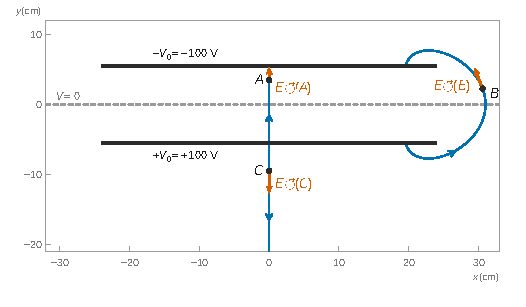
\includegraphics{figures/q11-lignes-de-champ.pdf}
\caption*{Figure 1 --- lignes de champ et champ électrique en A, B et C, orientés
de l'armature + (en bas) vers l'armature − (en haut) ; longueurs des
vecteurs indicatives}
\end{figure}

\textbf{Q12.} La densité volumique d'énergie électrique vaut

\equationajustee{\boxed{u_E=\frac{\varepsilon_0E^2}{2}}}

Avec un champ uniforme \(E=U/d\) localisé dans le volume \(\ell^2d\) :

\equationajustee{\begin{aligned}
U_E&=\frac{\varepsilon_0}{2}\frac{U^2}{d^2}\,\ell^2d\\
&=\frac12\,\frac{\varepsilon_0\ell^2}{d}\,U^2.
\end{aligned}}

L'identification avec \(U_E=\frac12C_0U^2\) donne

\equationajustee{\boxed{C_0=\frac{\varepsilon_0\ell^2}{d}}}

Pour le condensateur de la figure 5 :

\equationajustee{\begin{aligned}
C_0&=\frac{8{,}85\times10^{-12}\times0{,}48^2}{0{,}11}\\
&=1{,}85\times10^{-11}\ \text{F}\\
&=\boxed{18{,}5\ \text{pF}}
\end{aligned}}

\textbf{Q13.} À tension \(U\) fixée, la figure montre que le champ intérieur reste pratiquement égal à \(U/d\). Mais il existe aussi un champ non nul à l'extérieur des armatures (les équipotentielles s'y prolongent).

Ce champ stocke une énergie positive supplémentaire \(\iiint\varepsilon_0E^2/2\,\mathrm{d}\tau\). Donc \(U_{E,\text{\text{réel}}}>\frac12C_0U^2\), et comme \(C_{\text{\text{réel}}}=2U_{E,\text{\text{réel}}}/U^2\) :

\equationajustee{\boxed{C_{\text{\text{réel}}}>C_0}}

(On peut aussi dire que les lignes de champ extérieures partent de charges supplémentaires portées par les faces externes et les bords, d'où \(Q>C_0U\).)

\textbf{Q14.} On a \(\dfrac{C_{\text{\text{réel}}}-C_0}{C_0}=\kappa\left(\dfrac{d}{\ell}\right)^\beta\), donc \(y=\ln\kappa+\beta x\). L'identification avec la droite \(y=0{,}927x+0{,}819\) donne

\equationajustee{\boxed{\beta\approx0{,}93}}

\equationajustee{\boxed{\kappa=e^{0{,}819}\approx2{,}27}}

Pour la figure 5, \(d/\ell=11/48=0{,}229\), et \((d/\ell)^\beta=e^{0{,}927\ln0{,}229}=0{,}255\) :

\equationajustee{\begin{aligned}
C_{\text{\text{réel}}}&=C_0(1+2{,}27\times0{,}255)\\
&=1{,}58\,C_0
\end{aligned}}

\equationajustee{\boxed{C_{\text{\text{réel}}}\approx29\ \text{pF}}}

\textbf{Q15.} La seule loi fournie est \texttt{np.random.uniform(\allowbreak{}a,\allowbreak{}b)\allowbreak{}}. Une loi uniforme sur \([y_j-\Delta,\,y_j+\Delta]\) a un écart-type \(\Delta/\sqrt3\). Il faut donc \(\Delta=u_y\sqrt3\) pour simuler l'incertitude-type \(u_y\) :

\begin{lstlisting}[language=Python]
    for j in range(len(x)):                                          # ligne 19
        Y_i.append(np.random.uniform(y[j]-u_y*np.sqrt(3), y[j]+u_y*np.sqrt(3)))  # ligne 20
    a_i,b_i = np.polyfit(x, Y_i, 1)                                  # ligne 21
\end{lstlisting}

\emph{Lignes 30 et 31.} L'ordonnée à l'origine est \(b=\ln\kappa\), donc \(\kappa=e^b\). On prend pour \(\kappa\) l'image de la valeur moyenne \(b_m\) : \(\kappa=e^{b_m}\) (ligne 30). L'incertitude se propage par linéarisation, car \(u_b\ll1\) :

\equationajustee{\begin{aligned}
u_\kappa&=\left|\frac{\mathrm{d}\kappa}{\mathrm{d}b}\right|u_b\\
&=e^{b_m}u_b\\
&=\kappa\,u_b\quad\text{(ligne 31)}.
\end{aligned}}

L'incertitude absolue sur \(b\) est l'incertitude relative sur \(\kappa\). Pour \(\beta=a\), aucune transformation n'est nécessaire.

(Contrôle : avec les dix points du code, la simulation donne \(\beta\approx0{,}865\pm0{,}023\) et \(\kappa\approx2{,}21\pm0{,}05\). Ces valeurs diffèrent légèrement de la droite imprimée sur la figure 6, mais cela ne change rien à ce qui est demandé.)

\hypertarget{ii-couplage-magnuxe9tique}{%
\subsection{II --- Couplage magnétique}\label{ii-couplage-magnuxe9tique}}

\textbf{Q16.} On oriente les flux par les courants \(\underline{i_e}\) et \(\underline{i_s}\). Le premier entre dans \(L_1\) par le haut, le second sort de \(L_2\) par le haut vers \(C_2\). Le couplage \(M\) est positif pour ces orientations. Les flux propres et mutuels s'écrivent :

\equationajustee{\begin{aligned}
\phi_1&=L_1i_e+Mi_s\\
\phi_2&=L_2i_s+Mi_e
\end{aligned}}

La bobine \(L_1\) est en convention récepteur pour \(i_e\). La bobine \(L_2\) est en convention générateur pour \(i_s\). Les lois des mailles donnent :

\equationajustee{\boxed{\begin{aligned}\underline{u_e}&=\left(jL_1\omega+\frac{1}{jC_1\omega}\right)\underline{i_e}+jM\omega\,\underline{i_s}\\ \underline{u_s}&=-\left(jL_2\omega+\frac{1}{jC_2\omega}\right)\underline{i_s}-jM\omega\,\underline{i_e}\end{aligned}}}

Si \(L_1C_1\omega^2=L_2C_2\omega^2=1\), les termes \(j(L\omega-1/(C\omega))\) s'annulent :

\equationajustee{\boxed{\underline{u_e}=jM\omega\,\underline{i_s}}}

\equationajustee{\boxed{\underline{u_s}=-jM\omega\,\underline{i_e}}}

\emph{Rôle des condensateurs.} Chacun compense, à la fréquence de travail, la réactance de la bobine avec laquelle il est en série (résonance série). Les réactances propres \(L_1\omega\) et \(L_2\omega\), grandes devant \(M\omega\), ne limitent plus les courants. Le générateur voit une charge purement résistive (facteur de puissance égal à 1), et le transfert est maximal à tension imposée.

Avec \(\omega=2\pi\times1{,}20\times10^5=7{,}54\times10^5\ \text{rad}\cdot\text{s}^{-1}\) :

\equationajustee{\begin{aligned}
C_1&=\frac{1}{L_1\omega^2}\\
&=\frac{1}{50\times10^{-6}\times(7{,}54\times10^5)^2}
\end{aligned}}

\equationajustee{\boxed{C_1\approx35\ \text{nF}}}

On note aussi \(M=\eta\sqrt{L_1L_2}=27{,}1\ \mu\text{H}\), d'où \(M\omega=20{,}4\ \Omega\).

\textbf{Q17.} La batterie impose \(\underline{u_s}=R\,\underline{i_s}\). Donc :

\equationajustee{\begin{aligned}
\underline{i_s}&=-j\frac{M\omega}{R}\underline{i_e}\\
\underline{u_s}&=-jM\omega\,\underline{i_e}\\
\underline{u_e}&=jM\omega\,\underline{i_s}\\
&=\frac{(M\omega)^2}{R}\underline{i_e}
\end{aligned}}

\emph{Diagramme de Fresnel} (\(\underline{i_e}\) en référence, sur l'axe réel) :

\begin{itemize}
\tightlist
\item
  \(\underline{u_e}\) est colinéaire à \(\underline{i_e}\), de même sens : le générateur voit la résistance \(R_{\text{eq}}=(M\omega)^2/R=41{,}8\ \Omega\) ;
\item
  \(\underline{i_s}\) et \(\underline{u_s}\) sont colinéaires entre eux, en quadrature retard (\(-\pi/2\)) sur le courant primaire.
\end{itemize}

\begin{figure}[H]
\centering
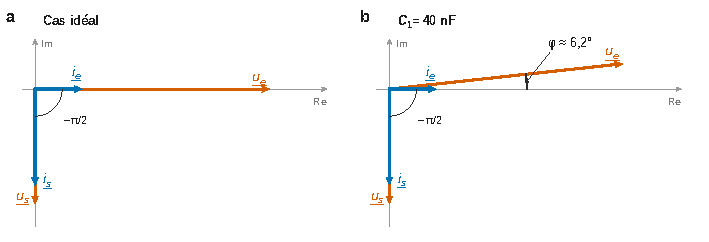
\includegraphics{figures/q17-q18-diagrammes-fresnel.pdf}
\caption*{Figure 2 --- diagrammes de Fresnel du coupleur, i\_e en référence : (a)
cas idéal, (b) C₁ = 40 nF, où u\_e prend 6,2° d'avance}
\end{figure}

Numériquement : \(I_{e,\text{eff}}=U_{e,\text{eff}}/R_{\text{eq}}=0{,}215\) A et \(I_{s,\text{eff}}=U_{e,\text{eff}}/(M\omega)=0{,}440\) A. On en tire \(U_{s,\text{eff}}=4{,}40\) V. La puissance transférée vaut

\equationajustee{\begin{aligned}
P&=\frac{U_{s,\text{eff}}^2}{R}\\
&=\frac{R\,U_{e,\text{eff}}^2}{(M\omega)^2}
\end{aligned}}

\equationajustee{\boxed{P\approx1{,}9\ \text{W}}}

Elle est égale à \(U_{e,\text{eff}}I_{e,\text{eff}}\) : bobines et condensateurs ne consomment rien.

\textbf{Q18.} \emph{Hypothèses} : seul \(C_1\) change, le secondaire reste accordé, \(U_{e,\text{eff}}=9\) V est imposée. Le primaire garde une réactance résiduelle

\equationajustee{\begin{aligned}
X_1&=L_1\omega-\frac{1}{C_1\omega}\\
&=37{,}70-33{,}16\\
&=4{,}54\ \Omega\ (\text{inductive}).
\end{aligned}}

La relation \(\underline{i_s}=-j(M\omega/R)\underline{i_e}\) est inchangée, et \(\underline{u_e}=\left(R_{\text{eq}}+jX_1\right)\underline{i_e}\).

\emph{Diagramme de Fresnel} : \(\underline{i_s}\) et \(\underline{u_s}\) restent en quadrature retard sur \(\underline{i_e}\). Mais \(\underline{u_e}\) est maintenant \textbf{en avance} sur \(\underline{i_e}\) de

\equationajustee{\begin{aligned}
\varphi&=\arctan\frac{X_1}{R_{\text{eq}}}\\
&=\arctan\frac{4{,}54}{41{,}8}\\
&\approx6{,}2^\circ.
\end{aligned}}

À \(U_{e,\text{eff}}\) fixée, tous les courants diminuent dans le rapport \(R_{\text{eq}}/|R_{\text{eq}}+jX_1|=0{,}994\).

\emph{Puissance} :

\equationajustee{\begin{aligned}
P'&=\frac{R_{\text{eq}}U_{e,\text{eff}}^2}{R_{\text{eq}}^2+X_1^2}\\
&=\frac{P}{1+(X_1/R_{\text{eq}})^2}\\
&=1{,}92\ \text{W}
\end{aligned}}

\equationajustee{\boxed{\frac{\Delta P}{P}\approx-1{,}2\ \%}}

La perte est du second ordre en \(X_1/R_{\text{eq}}\). Un désaccord de 14 \% sur \(C_1\) est donc peu pénalisant, parce que la résistance ramenée (42 Ω) est grande devant \(X_1\). Le facteur de puissance passe à \(\cos6{,}2^\circ=0{,}994\).

\hypertarget{partie-c-mesures-de-puissances}{%
\section{Partie C --- Mesures de puissances}\label{partie-c-mesures-de-puissances}}

\hypertarget{i-multiplicateur-uxe0-effet-hall}{%
\subsection{I --- Multiplicateur à effet Hall}\label{i-multiplicateur-uxe0-effet-hall}}

\textbf{Q19.} La force de Lorentz vaut

\equationajustee{\boxed{\vec f_{L,i}=q_i\left(\vec E+\vec v_i\wedge\vec B_0\right)}}

En régime stationnaire, \(m_i\,\mathrm{d}\vec v_{i,s}/\mathrm{d}t=\vec0\) (poids négligé), donc

\equationajustee{q_i(\vec E+\vec v_{i,s}\wedge\vec B_0)-\lambda_i\vec v_{i,s}=\vec0,}

soit

\equationajustee{\vec v_{i,s}=\frac{q_i}{\lambda_i}\left(\vec E+\vec v_{i,s}\wedge\vec B_0\right)}

\equationajustee{\boxed{\mu_i=\frac{q_i}{\lambda_i}}}

(la mobilité a le signe de la charge : \(\mu_e<0\)).

\textbf{Q20.} On a \(\vec j=-n_ee\,\vec v_{e,s}\), donc \(\vec v_{e,s}=-\vec j/(n_ee)\). En reportant dans Q19 :

\equationajustee{\begin{aligned}
-\frac{\vec j}{n_ee}&=\mu_e\left(\vec E-\frac{\vec j\wedge\vec B_0}{n_ee}\right)\\
\vec j&=-n_ee\mu_e\left(\vec E-\frac{1}{n_ee}\,\vec j\wedge\vec B_0\right),
\end{aligned}}

\equationajustee{\boxed{\gamma=-n_ee\mu_e>0}}

\equationajustee{\boxed{K_H=-\frac{1}{n_ee}}}

\textbf{Q21.}

\equationajustee{\begin{aligned}
n_e&=\frac{1}{e|K_H|}\\
&=\frac{1}{1{,}602\times10^{-19}\times9{,}98\times10^{-5}}
\end{aligned}}

\equationajustee{\boxed{n_e\approx6{,}3\times10^{22}\ \text{m}^{-3}}}

\equationajustee{\begin{aligned}
\gamma&=n_ee|\mu_e|\\
&=\frac{|\mu_e|}{|K_H|}\\
&=\frac{3{,}3}{9{,}98\times10^{-5}}
\end{aligned}}

\equationajustee{\boxed{\gamma\approx3{,}3\times10^4\ \text{S}\cdot\text{m}^{-1}}}

Pour le cuivre, \(\gamma\approx6\times10^7\ \text{S}\cdot\text{m}^{-1}\) et \(n_e\approx10^{29}\ \text{m}^{-3}\). InAs est environ \(2\times10^3\) fois moins conducteur et compte \(10^6\) fois moins de porteurs.

On utilise un semi-conducteur parce que la tension de Hall est proportionnelle à \(|K_H|=1/(n_ee)\). À courant et champ égaux, elle y est environ \(10^6\) fois plus grande que dans un métal, donc mesurable.

\textbf{Q22.} Avec \(\vec j=j_x\vec e_x\) et \(\vec B_0=B_0\vec e_z\), on a \(\vec j\wedge\vec B_0=-j_xB_0\vec e_y\). Comme \(j_y=0\), la projection sur \(\vec e_y\) donne

\equationajustee{0=\gamma(E_y-K_HB_0j_x),}

\equationajustee{\boxed{E_y=K_HB_0\,j_x}}

Plaquette : longueur \(a\) selon \(\vec e_x\), largeur \(b\) selon \(\vec e_y\). Son épaisseur \(c\) est selon \(\vec e_z\) (la plaquette doit tenir dans l'entrefer de 2 mm).

Le point \(C\) est sur la face \(y=0\). Le point \(D\) est sur la face \(y=b\). Avec \(I=j_xbc\) :

\begin{figure}[H]
\centering
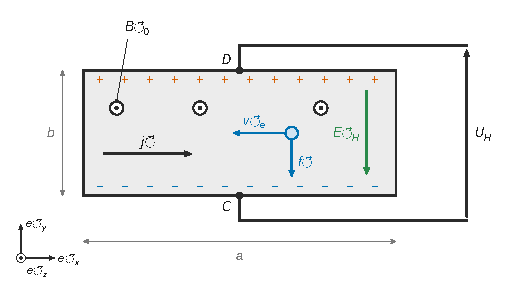
\includegraphics{figures/q22-effet-hall-plaquette.pdf}
\caption*{Figure 3 --- effet Hall, vue de dessus : B₀ sortant, électrons déviés
vers la face y = 0 (C), champ de Hall de D vers C}
\end{figure}

\equationajustee{\begin{aligned}
U_H&=V(D)-V(C)\\
&=-\int_0^bE_y\,\mathrm{d}y\\
&=-K_HB_0j_xb
\end{aligned}}

\equationajustee{\boxed{U_H=-\frac{K_HB_0I}{c}=\frac{B_0I}{n_eec}}}

La loi d'Ohm dans la plaquette donne \(u=E_xa\) et \(j_x=\gamma E_x\), donc \(I=\gamma\dfrac{bc}{a}u\), et

\equationajustee{U_H=-K_H\gamma\frac{b}{a}B_0u}

\equationajustee{\boxed{A_H=-K_H\gamma\frac{b}{a}=-\mu_e\frac{b}{a}}}

car \(K_H\gamma=\mu_e\). Numériquement, \(A_H=3{,}3\times3/5\approx2{,}0\ \text{T}^{-1}\) (dimension d'une mobilité).

\textbf{Q23.} \emph{Champ dans l'entrefer.} Le théorème d'Ampère sur la ligne moyenne du tore, qui enlace une fois le fil, donne

\equationajustee{H_{\text{fer}}(l-\ell_e)+H_e\ell_e=i.}

La conservation du flux (fuites négligées) impose \(B_{\text{fer}}=B_e=B_0\). On a de plus \(H_{\text{fer}}=B_0/(\mu_0\mu_r)\) et \(H_e=B_0/\mu_0\) :

\equationajustee{\begin{aligned}
B_0&=\frac{\mu_0\,i}{\ell_e+(l-\ell_e)/\mu_r}\\
&\approx\frac{\mu_0\,i}{\ell_e}
\end{aligned}}

car \((l-\ell_e)/\mu_r=4{,}8\times10^{-7}\) m \(\ll\ell_e=2\times10^{-3}\) m.

\emph{Produit.} D'après Q22, \(U_H=A_HB_0u\), donc

\equationajustee{\boxed{U_H=\alpha\,u\,i}}

\equationajustee{\boxed{\alpha=\frac{A_H\mu_0}{\ell_e}=-\frac{\mu_e\,b\,\mu_0}{a\,\ell_e}}}

\equationajustee{\begin{aligned}
\alpha&=\frac{2{,}0\times1{,}26\times10^{-6}}{2\times10^{-3}}\\
&\approx\boxed{1{,}2\times10^{-3}\ \text{A}^{-1}}
\end{aligned}}

\(U_H\) est proportionnelle à la puissance \(u\,i\).

\emph{Protocole de mesure de \(\alpha\).}

\begin{enumerate}
\def\labelenumi{\arabic{enumi}.}
\tightlist
\item
  Alimenter la plaquette par une tension continue réglable \(u\), mesurée au voltmètre. La résistance de la plaquette vaut \(a/(\gamma bc)\approx0{,}1\ \Omega\) : on limite \(u\) à quelques dizaines de mV pour éviter l'échauffement.
\item
  Faire passer dans le fil un courant continu réglable \(i\), mesuré à l'ampèremètre.
\item
  Mesurer \(U_H\) entre \(D\) et \(C\) avec un millivoltmètre de grande impédance d'entrée.
\item
  Éliminer la tension de décalage (contacts mal alignés) : inverser \(i\) et prendre \([U_H(i)-U_H(-i)]/2\).
\item
  Relever une dizaine de couples \((u,i)\), puis tracer \(U_H\) en fonction de \(u\,i\). Vérifier l'alignement sur une droite passant par l'origine. La pente, obtenue par régression linéaire, donne \(\alpha\), et son incertitude s'évalue par Monte-Carlo comme en Q15.
\end{enumerate}

\hypertarget{ii-le-cristal}{%
\subsection{II --- Le cristal}\label{ii-le-cristal}}

\textbf{Q24.} In\(^{3+}\) (cfc) : \(8\times\frac18+6\times\frac12=4\). La maille compte 8 sites tétraédriques intérieurs, dont la moitié est occupée par As\(^{3-}\) : 4. \textbf{La maille contient 4 In\(^{3+}\) et 4 As\(^{3-}\) (4 motifs InAs).}

La charge totale vaut \(4\times(+3e)+4\times(-3e)=0\) : le cristal est électriquement neutre. Un site tétraédrique est entouré de 4 In\(^{3+}\) : \textbf{la coordinence As--In vaut 4} (et In--As aussi, par stœchiométrie : structure blende).

\textbf{Q25.} Le site tétraédrique est le centre d'un cube d'arête \(a/2\). Le contact anion-cation se fait selon la demi-diagonale de ce petit cube : \(r_{\text{In}^{3+}}+r_{\text{As}^{3-}}=\dfrac{a\sqrt3}{4}\).

\equationajustee{\boxed{a=\frac{4\left(r_{\text{In}^{3+}}+r_{\text{As}^{3-}}\right)}{\sqrt3}}}

\equationajustee{\begin{aligned}
a&=\frac{4\times240}{\sqrt3}\ \text{pm}\\
&=\boxed{554\ \text{pm}}
\end{aligned}}

\equationajustee{\boxed{\rho_{\text{InAs}}=\frac{4(M_{\text{In}}+M_{\text{As}})}{{\mathcal{N}}_Aa^3}}}

\equationajustee{\begin{aligned}
\rho_{\text{InAs}}&=\frac{4\times189{,}7\times10^{-3}}{6{,}02\times10^{23}\times(5{,}54\times10^{-10})^3}\\
&=\boxed{7{,}4\times10^3\ \text{kg}\cdot\text{m}^{-3}}
\end{aligned}}

(La valeur réelle est d'environ \(5{,}7\times10^3\ \text{kg}\cdot\text{m}^{-3}\), avec \(a=606\) pm. Le modèle ionique de sphères tangentes est approximatif, car la liaison In--As est largement covalente.)

\hypertarget{iii-multiplicateur-numuxe9rique-uxe0-modulation-damplitude}{%
\subsection{III --- Multiplicateur numérique à modulation d'amplitude}\label{iii-multiplicateur-numuxe9rique-uxe0-modulation-damplitude}}

\textbf{Q26.} Le spectre de \(u\) est contenu dans \([0,F]\). Le critère de Nyquist-Shannon impose

\equationajustee{\boxed{f_e=\frac{1}{T_e}>2F}}

Sinon, il y a repliement de spectre.

\textbf{Q27.} Sur \([nT_e,(n+1)T_e]\), \(s_r(t)=-U_0+2U_0\dfrac{t-nT_e}{T_e}\).

Le comparateur reçoit \(u_{\text{ech}}=u_n\) sur l'entrée + et \(s_r\) sur l'entrée −. On a \(S=+V_{\text{sat}}\) tant que \(s_r<u_n\), c'est-à-dire au début de l'intervalle, puisque \(|u_n|<U_0\). La bascule a lieu quand \(-U_0+2U_0\alpha_n=u_n\) :

\equationajustee{\boxed{\alpha_n=\frac12\left(1+\frac{u_n}{U_0}\right)}}

\textbf{Q28.} L'ALI est idéal, avec une rétroaction sur l'entrée \(-\) : il fonctionne en régime linéaire, \(V_-=V_+=0\), et ses courants d'entrée sont nuls. Le courant \(i\) traverse \(R\), donc \(0-v_i=Ri\) :

\equationajustee{\boxed{v_i(t)=-R\,i(t)}}

\emph{Intérêt} : c'est un convertisseur courant-tension dont l'entrée est une masse virtuelle. Il présente une impédance d'entrée nulle (ampèremètre idéal), ne perturbe pas le circuit mesuré et délivre une tension image de \(i\) sous faible impédance de sortie.

\textbf{Q29.} L'ALI est en régime linéaire, avec \(V_+=V_-\) et des courants d'entrée nuls.

\begin{itemize}
\tightlist
\item
  \(K\) fermé (\(S>0\)) : \(V_+=0\). C'est un montage inverseur de gain \(-R/R\), donc \(v_{i,\text{mod}}=-v_{i,\text{ech}}\).
\item
  \(K\) ouvert (\(S<0\)) : aucun courant dans la résistance reliée à l'entrée +, donc \(V_+=v_{i,\text{ech}}=V_-\). Le courant dans la résistance d'entrée est nul, donc aussi dans la résistance de rétroaction, et \(v_{i,\text{mod}}=v_{i,\text{ech}}\).
\end{itemize}

\equationajustee{\boxed{v_{i,\text{mod}}=\begin{cases}-v_{i,\text{ech}}&\text{si }S>0\\ +v_{i,\text{ech}}&\text{si }S<0\end{cases}}}

\textbf{Q30.} Montage intégrateur inverseur : une résistance \(R_1\) entre \(v_e\) et l'entrée −, un condensateur \(C_1'\) entre l'entrée − et la sortie, l'entrée + à la masse.

\begin{figure}[H]
\centering
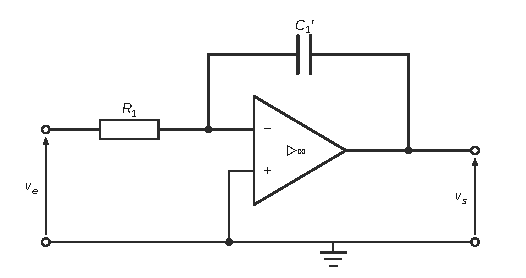
\includegraphics{figures/q30-integrateur-ali.pdf}
\caption*{Figure 4 --- montage intégrateur inverseur, R₁ en entrée et C₁′ en
contre-réaction, entrée + à la masse}
\end{figure}

Masse virtuelle : le courant \(v_e/R_1\) traverse le condensateur, donc

\equationajustee{\frac{v_e}{R_1}=-C_1'\frac{\mathrm{d}v_s}{\mathrm{d}t},}

\equationajustee{\boxed{v_s(t)=-\frac{1}{R_1C_1'}\int v_e\,\mathrm{d}t}}

avec \(\tau=R_1C_1'\). En pratique, on place une grande résistance en parallèle sur \(C_1'\) pour éviter la dérive vers la saturation.

\textbf{Q31.} Sur \(]nT_e,(n+1)T_e]\), \(v_{i,\text{ech}}=v_{i,n}=-Ri_n\) est constant. La tension modulée vaut \(-v_{i,n}\) pendant \(\alpha_nT_e\), puis \(+v_{i,n}\) pendant le reste de l'intervalle :

\equationajustee{\begin{aligned}
\int_{nT_e}^{(n+1)T_e}v_{i,\text{mod}}\,\mathrm{d}t&=v_{i,n}T_e(1-2\alpha_n)\\
&=-v_{i,n}T_e\frac{u_n}{U_0}.
\end{aligned}}

Donc \(v_{m,n}=\dfrac{v_{i,n}T_e}{\tau}\dfrac{u_n}{U_0}\), soit

\equationajustee{\boxed{v_{m,n}=-\frac{R\,T_e}{\tau\,U_0}\,u_n\,i_n}}

La tension obtenue est proportionnelle au produit \(u_ni_n\), avec une constante \(-RT_e/(\tau U_0)\) indépendante des signaux : c'est la puissance instantanée échantillonnée, à une constante près.

\textbf{Q32.} Pour \(\omega\to\infty\), \(\underline{H}\to1\). Pour \(\omega\to0\), le terme dominant du dénominateur est \(\dfrac{j}{(RC\omega)^3}\). Donc \(|\underline{H}|\sim(RC\omega)^3\to0\) (pente de +60 dB/décade). \textbf{C'est un filtre passe-haut d'ordre 3}, de gain unité à haute fréquence.

\textbf{Q33.} L'entrée + est à la masse, et \(v\) attaque l'entrée − à travers \(R\), avec \(R'\) en rétroaction : montage inverseur,

\equationajustee{\boxed{G=\frac{v_s}{v}=-\frac{R'}{R}}}

\(K'\) fermé : \(v_e=v_s\) et \(v=\underline{H}v_e\). L'amplificateur impose \(v_s=Gv\). Donc \(v_s=G\underline{H}\,v_s\). Un régime sinusoïdal d'amplitude non nulle exige

\equationajustee{\boxed{G\,\underline{H}(\omega_{\text{osc}})=1}}

\(G\) étant réel, \(\underline{H}\) doit l'être : \(6-\dfrac{1}{(RC\omega)^2}=0\), soit

\equationajustee{\boxed{\omega_{\text{osc}}=\frac{1}{\sqrt6\,RC}}}

Alors \(\underline{H}=\dfrac{1}{1-30}=-\dfrac{1}{29}\), et

\equationajustee{\boxed{G=-29}}

soit \(R'=29R\).

\textbf{Q34.} Le gain vaut \(|G|=R_{\text{com}}/R\). Pour que l'amplitude soit stable, il faut \(|G|>29\) aux faibles amplitudes (démarrage des oscillations) et \(|G|<29\) aux fortes amplitudes (limitation). Ainsi \(R_{\text{com}}\) doit \textbf{décroître} avec \(A_{\text{osc}}\).

L'expression 1) est décroissante, l'expression 2) croissante. Avec 2), on aurait même \(R_{\text{com}}<R_0=125\ \text{k}\Omega<29R=145\ \text{k}\Omega\) : les oscillations ne démarreraient pas.

\equationajustee{\boxed{R_{\text{com}}=R_0+\frac{r}{1+A_{\text{osc}}/V_0}\quad\text{(expression 1)}}}

En régime établi, \(R_{\text{com}}=29R\) :

\equationajustee{\begin{aligned}
r&=(29R-R_0)\left(1+\frac{A_{\text{osc}}}{V_0}\right)\\
&=(145-125)\times2{,}4\ \text{k}\Omega
\end{aligned}}

\equationajustee{\boxed{r=48\ \text{k}\Omega}}

(contrôle : \(R_0+r=173\ \text{k}\Omega>145\ \text{k}\Omega\), le démarrage est assuré).

\hypertarget{partie-d-accumulateur-lithium-air}{%
\section{Partie D --- Accumulateur lithium-air}\label{partie-d-accumulateur-lithium-air}}

\hypertarget{i-stabilituxe9-du-lithium}{%
\subsection{I --- Stabilité du lithium}\label{i-stabilituxe9-du-lithium}}

\textbf{Q35.} Les demi-équations sont \(\mathrm{Li^+_{(aq)}}+\mathrm{e^-}=\mathrm{Li_{(s)}}\) et \(2\mathrm{H^+_{(aq)}}+2\mathrm{e^-}=\mathrm{H_{2(g)}}\). Réaction bilan :

\equationajustee{\boxed{2\,\mathrm{Li_{(s)}}+2\,\mathrm{H^+_{(aq)}}=2\,\mathrm{Li^+_{(aq)}}+\mathrm{H_{2(g)}}}}

\equationajustee{\boxed{\Delta_rG^o=-2F\left[E^o(\mathrm{H^+/H_2})-E^o(\mathrm{Li^+/Li})\right]}}

\equationajustee{\begin{aligned}
\Delta_rG^o&=-2\times9{,}65\times10^4\times3{,}045\\
&\approx-5{,}88\times10^5\ \text{J}\cdot\text{mol}^{-1}
\end{aligned}}

\textbf{Q36.}

\equationajustee{\boxed{K^o=\exp\left(-\frac{\Delta_rG^o}{RT}\right)}}

\equationajustee{\begin{aligned}
\log K^o&=\frac{2\times3{,}045}{0{,}059}\\
&=103
\end{aligned}}

\equationajustee{\boxed{K^o\approx10^{103}}}

La réaction est totale. Sans blocage cinétique, le lithium serait entièrement oxydé au contact de la solution aqueuse (l'eau suffit) : autodécharge et destruction de l'électrode, dégagement de dihydrogène inflammable dans un milieu qui s'échauffe, d'où un risque d'incendie ou d'explosion.

\textbf{Q37.} \(\mathrm{H^+}\) est un réactif. Augmenter le pH diminue \([\mathrm{H^+}]\), donc augmente le quotient \(Q_r=\dfrac{[\mathrm{Li^+}]^2\,p(\mathrm{H_2})/p^o}{[\mathrm{H^+}]^2}\). Alors \(\Delta_rG=\Delta_rG^o+RT\ln Q_r\) augmente : la réaction est moins favorisée.

De façon équivalente, \(E(\mathrm{H^+/H_2})\) diminue avec le pH alors que \(E(\mathrm{Li^+/Li})\) n'en dépend pas.

\textbf{Q38.}

\equationajustee{\boxed{E_1=-3{,}045+0{,}059\log[\mathrm{Li^+}]}}

\equationajustee{\begin{aligned}
E_2&=\frac{0{,}059}{2}\log\frac{[\mathrm{H^+}]^2}{p(\mathrm{H_2})/p^o}\\
&=\boxed{-0{,}059\,\mathrm{pH}}
\end{aligned}}

\equationajustee{\Delta_rG=-2F(E_2-E_1)}

\equationajustee{\boxed{\Delta_rG=\Delta_rG^o+2F\times0{,}059\left(\mathrm{pH}+\log[\mathrm{Li^+}]\right)}}

Pour \(\mathrm{pH}=14\) et \([\mathrm{Li^+}]=1{,}0\ \text{mol}\cdot\text{L}^{-1}\) :

\equationajustee{\begin{aligned}
\Delta_rG&=-588+2\times9{,}65\times10^4\times0{,}059\times14\times10^{-3}\\
&=-588+159
\end{aligned}}

\equationajustee{\boxed{\Delta_rG\approx-4{,}3\times10^2\ \text{kJ}\cdot\text{mol}^{-1}}}

\textbf{La réaction n'est pas évitée en milieu basique} : il faudrait \(\mathrm{pH}\approx52\) pour annuler \(\Delta_rG\). Seule une protection cinétique (le revêtement) peut préserver le lithium.

\hypertarget{ii-fonctionnement-de-laccumulateur}{%
\subsection{II --- Fonctionnement de l'accumulateur}\label{ii-fonctionnement-de-laccumulateur}}

\textbf{Q39.} Électrode de nickel (électrode à dioxygène, en milieu basique) :

\equationajustee{\boxed{\mathrm{O_2}+2\mathrm{H_2O}+4\mathrm{e^-}=4\mathrm{HO^-}}}

Le potentiel est celui du couple \(\mathrm{O_2/H_2O}\) :

\equationajustee{\begin{aligned}
E_{\mathrm{O_2}}&=1{,}23+\frac{0{,}059}{4}\log\left(\frac{p(\mathrm{O_2})}{p^o}[\mathrm{H^+}]^4\right)\\
&=1{,}23+0{,}0148\log0{,}2-0{,}059\times14
\end{aligned}}

\equationajustee{\boxed{E_{\mathrm{O_2}}\approx0{,}39\ \text{V}}}

\equationajustee{E_{\mathrm{Li}}=-3{,}045+0{,}059\log0{,}1}

\equationajustee{\boxed{E_{\mathrm{Li}}\approx-3{,}10\ \text{V}}}

\equationajustee{\boxed{e=E_{\mathrm{O_2}}-E_{\mathrm{Li}}\approx3{,}5\ \text{V}}}

(La valeur de 3 V du tableau 1 tient compte des surpotentiels et des chutes ohmiques.)

\textbf{Q40.} En décharge (document réponse) :

\begin{itemize}
\tightlist
\item
  électrode de lithium : \textbf{anode}, oxydation \(\mathrm{Li}=\mathrm{Li^+}+\mathrm{e^-}\), \textbf{pôle \(-\)} ;
\item
  électrode de carbone poreux : \textbf{cathode}, réduction \(\mathrm{O_2}+2\mathrm{H_2O}+4\mathrm{e^-}=4\mathrm{HO^-}\), \textbf{pôle \(+\)} ;
\item
  électrons : dans le circuit extérieur, du lithium vers le carbone, à travers \(R\) ;
\item
  courant : dans le circuit extérieur, du carbone vers le lithium ;
\item
  ions : dans l'électrolyte, \(\mathrm{Li^+}\) migre vers l'électrode de carbone, \(\mathrm{HO^-}\) vers l'électrode de lithium.
\end{itemize}

\begin{figure}[H]
\centering
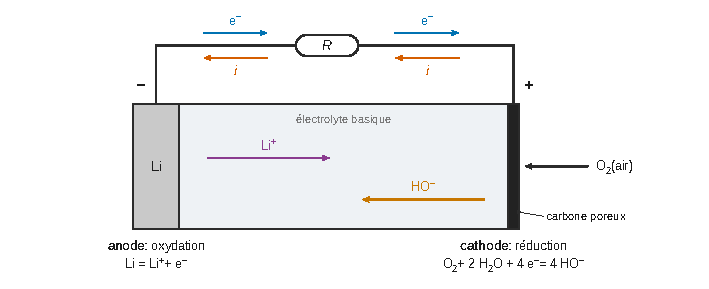
\includegraphics{figures/q40-accumulateur-decharge.pdf}
\caption*{Figure 5 --- accumulateur lithium-air en décharge : polarités,
électrons, courant, migration des ions et réactions aux électrodes}
\end{figure}

\textbf{Q41.} LiOH précipite là où le produit \([\mathrm{Li^+}][\mathrm{HO^-}]\) est maximal. \textbf{En décharge}, \(\mathrm{HO^-}\) est produit à l'électrode à dioxygène (carbone poreux), vers laquelle migrent les ions \(\mathrm{Li^+}\) : \textbf{le précipité se forme au voisinage de l'électrode à dioxygène poreuse}. En charge, \(\mathrm{HO^-}\) y est au contraire consommé.

\emph{Problème} : le solide obstrue les pores et recouvre la surface active. La diffusion de \(\mathrm{O_2}\) est bloquée, la résistance interne et les surpotentiels augmentent, et la capacité diminue de façon irréversible.

\textbf{Q42.} \emph{Hypothèses} : décharge complète correspondant à l'autonomie maximale, rendement faradique de 1, volume d'électrolyte assimilé à \(V=W/W_{\max}\), et tout \(\mathrm{Li^+}\) au-delà de \(c_{\max}\) précipite.

\begin{itemize}
\item
  Énergie : \(W=6\times15=90\ \text{kW}\cdot\text{h}=3{,}24\times10^8\) J.
\item
  Les \(N=400/3\approx133\) cellules sont en série et sont traversées par la même charge :

  \equationajustee{\begin{aligned}
  Q&=\frac{W}{U}\\
  &=\frac{3{,}24\times10^8}{400}\\
  &=8{,}1\times10^5\ \text{C}.
  \end{aligned}}

  Chaque cellule produit \(Q/F=8{,}4\) mol de \(\mathrm{Li^+}\). Au total :

  \equationajustee{\begin{aligned}
  n&=N\frac{Q}{F}\\
  &=\frac{W}{e_{\text{cell}}F}\\
  &=\frac{3{,}24\times10^8}{3\times9{,}65\times10^4}\\
  &\approx1{,}12\times10^3\ \text{mol}.
  \end{aligned}}
\item
  Volume : \(V=90/2{,}2=41\) L. La quantité restant dissoute vaut au plus \(c_{\max}V=5{,}25\times41\approx2{,}1\times10^2\) mol.
\item
  Avec \(M(\mathrm{LiOH})=23{,}9\ \text{g}\cdot\text{mol}^{-1}\) :
\end{itemize}

\equationajustee{m=(1119-215)\times23{,}9\ \text{g}}

\equationajustee{\boxed{m\approx22\ \text{kg}}}

(Si l'on néglige la fraction dissoute, on obtient la borne supérieure de \(27\) kg.) C'est considérable pour une batterie d'une quarantaine de litres.

\textbf{Q43.} \textbf{C'est à la charge qu'il faut une réaction rapide.} En charge, \(\mathrm{O_2}\) est produit et se dégage (flèche montante sur la figure 15a) : il n'est pas nécessaire que l'électrode soit poreuse.

En revanche, l'oxydation de \(\mathrm{HO^-}\) en \(\mathrm{O_2}\) présente un fort surpotentiel (système lent). L'électrode de nickel, électrocatalytique et stable aux potentiels élevés (le carbone y serait corrodé), rend la réaction rapide. On réduit ainsi la tension de charge, on améliore le rendement et on raccourcit la recharge.

En décharge, \(\mathrm{O_2}\) est consommé et doit venir de l'air : l'étape limitante est son transport, d'où \textbf{l'électrode de carbone poreux}, à grande surface, à travers laquelle diffuse le dioxygène.

\textbf{Q44.} Le courant change de sens entre la charge et la décharge. On relie le circuit extérieur aux deux électrodes à dioxygène par \textbf{deux diodes montées en sens opposés} :

\begin{figure}[H]
\centering
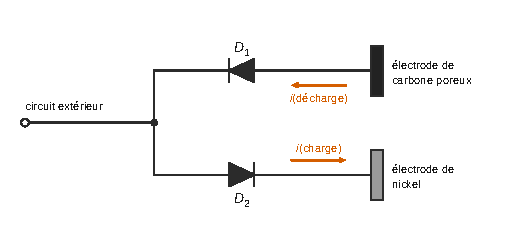
\includegraphics{figures/q44-diodes-tete-beche.pdf}
\caption*{Figure 6 --- interrupteur K réalisé par deux diodes en sens opposés, D₁
passante en décharge et D₂ en charge}
\end{figure}

En décharge, le courant sort de l'accumulateur par l'électrode à dioxygène (pôle \(+\)) : \(D_1\), orientée de l'électrode de carbone vers le circuit extérieur, conduit, et \(D_2\) est bloquée. En charge, le courant entre par l'électrode à dioxygène : \(D_2\), orientée du circuit extérieur vers le nickel, conduit, et \(D_1\) est bloquée.

La commutation est spontanée. On choisira des diodes à faible seuil (Schottky), car une chute de \(0{,}6\) V n'est pas négligeable devant 3 V.

\end{document}
